%% ma: L12-B17-0001
%% lop: 12
%% chuong: 5
%% bai: 17
%% dang: 12.17.1
%% loai: DS
%% muc: [TH, VD, VD, VD]
%% dap_an: "ĐSĐĐ"
%% nguon: "0. ĐỀ THAM KHẢO TN THPT 2025.pdf (D00), Phần II Câu 4"
%% kien_thuc: "Bài 15 (phương trình tham số của đường thẳng), Bài 17 (mặt cầu, giao của đường thẳng và mặt cầu); chuyển động thẳng đều (thời gian tỉ lệ với quãng đường)"
%% ghi_chu: "Hình dựng lại theo số liệu của đề: mặt cắt qua O chứa đường thẳng MN (khoảng cách từ O đến MN là 4√5 ≈ 8,94), tỉ lệ đúng; ý a) đề gốc đúng; đáp án gốc khớp"
%% trang_thai: cho-duyet
%% ly_do: "Dạng toán mới đề xuất 12.17.1, chờ giáo viên duyệt"
\begin{ex}
Các thiên thạch có đường kính lớn hơn $140$ m và có thể lại gần Trái Đất ở khoảng cách nhỏ hơn $7\,500\,000$ km được coi là những vật thể có khả năng va chạm gây nguy hiểm cho Trái Đất. Để theo dõi những thiên thạch này, người ta đã thiết lập các trạm quan sát các vật thể bay gần Trái Đất. Giả sử có một hệ thống quan sát có khả năng theo dõi các vật thể ở độ cao không vượt quá $6\,600$ km so với mực nước biển. Coi Trái Đất là khối cầu có bán kính $6\,400$ km. Chọn hệ trục tọa độ $Oxyz$ trong không gian có gốc $O$ tại tâm Trái Đất và đơn vị độ dài trên mỗi trục tọa độ là $1000$ km. Một thiên thạch (coi như một hạt) chuyển động với tốc độ không đổi theo một đường thẳng từ điểm $M(6;20;0)$ đến điểm $N(-6;-12;16)$.
\begin{center}
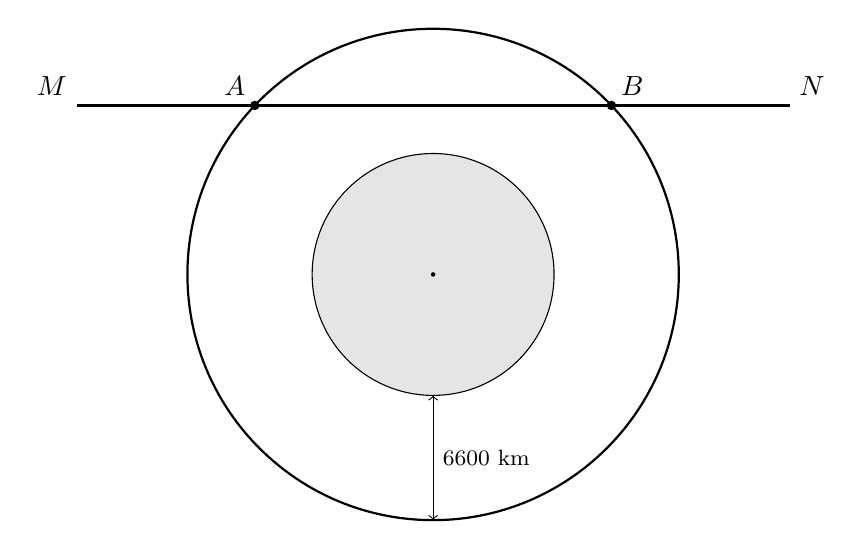
\begin{tikzpicture}[scale=.24]
  \def\R{13}\def\r{6.4}\def\h{8.944}\def\w{18.868}
  \draw[thick] (0,0) circle (\R);
  \draw[fill=gray!20] (0,0) circle (\r);
  \fill (0,0) circle (.12);
  \draw[thick] (-\w,\h)--(\w,\h);
  \path (-\w,\h) node[above left]{$M$} (\w,\h) node[above right]{$N$};
  \fill (-9.434,\h) circle (.25) (9.434,\h) circle (.25);
  \path (-9.434,\h) node[above left]{$A$} (9.434,\h) node[above right]{$B$};
  \draw[<->] (0,-\R) -- (0,-\r) node[midway,right,font=\footnotesize]{$6600$ km};
\end{tikzpicture}
\end{center}
\choiceTF
{\True Đường thẳng $MN$ có phương trình tham số là $\begin{cases}x=6+3t\\ y=20+8t\\ z=-4t\end{cases}$ $(t\in\mathbb R)$.}
{Vị trí đầu tiên thiên thạch di chuyển vào phạm vi theo dõi của hệ thống quan sát là điểm $A(-3;-4;12)$.}
{\True Khoảng cách giữa vị trí đầu tiên và vị trí cuối cùng mà thiên thạch di chuyển trong phạm vi theo dõi của hệ thống quan sát là $18\,900$ km (kết quả làm tròn đến hàng trăm theo đơn vị ki-lô-mét).}
{\True Nếu thời gian di chuyển của thiên thạch trong phạm vi theo dõi của hệ thống quan sát là $3$ phút thì thời gian nó di chuyển từ $M$ đến $N$ là $6$ phút.}
\loigiai{$\overrightarrow{MN}=(-12;-32;16)=-4(3;8;-4)$, đường thẳng $MN$ qua $M(6;20;0)$ có vectơ chỉ phương $(3;8;-4)$ nên a) đúng. Khi $t$ giảm từ $0$ đến $-4$ điểm chuyển động từ $M$ đến $N$.
Phạm vi theo dõi là hình cầu tâm $O$ bán kính $6{,}4+6{,}6=13$ (đơn vị $1000$ km). Thay vào $x^2+y^2+z^2=169$: $(6+3t)^2+(20+8t)^2+16t^2=169\Leftrightarrow89t^2+356t+267=0\Leftrightarrow t=-1$ hoặc $t=-3$.
Vị trí đầu tiên (gặp trước khi đi từ $M$) ứng với $t=-1$: $A(3;12;4)$, nên b) sai. Vị trí cuối cùng ứng với $t=-3$: $B(-3;-4;12)$.
$AB=\sqrt{(-6)^2+(-16)^2+8^2}=2\sqrt{89}\approx18{,}87$ nghìn km $\approx18\,900$ km: c) đúng.
$MN=4\sqrt{89}=2AB$ và thiên thạch chuyển động với tốc độ không đổi nên thời gian đi $MN$ gấp đôi thời gian đi $AB$, tức $6$ phút: d) đúng.}
\end{ex}
